\documentclass[a4]{article}
\pagestyle{myheadings}

%%%%%%%%%%%%%%%%%%%
% Packages/Macros %
%%%%%%%%%%%%%%%%%%%
\usepackage{mathrsfs}



\usepackage{fancyhdr}
\pagestyle{fancy}
\lhead{}
\chead{}
\rhead{}
\lfoot{}
\cfoot{} 
\rfoot{\normalsize\thepage}
\renewcommand{\headrulewidth}{0pt}
\renewcommand{\footrulewidth}{0pt}
\newcommand{\RomanNumeralCaps}[1]
    {\MakeUppercase{\romannumeral #1}}

\usepackage{amssymb,latexsym}  % Standard packages
\usepackage[utf8]{inputenc}
\usepackage[russian]{babel}
\usepackage{MnSymbol}
\usepackage{mathrsfs}
\usepackage{amsmath,amsthm}
\usepackage{indentfirst}
\usepackage{graphicx}%,vmargin}
\usepackage{graphicx}
\graphicspath{{pictures/}} 
\usepackage{verbatim}
\usepackage{color}
\usepackage[nottoc,numbib]{tocbibind}
\usepackage{float}

\usepackage{listings}
\definecolor{codegreen}{rgb}{0,0.6,0}
\definecolor{codegray}{rgb}{0.5,0.5,0.5}
\definecolor{codepurple}{rgb}{0.58,0,0.82}
\definecolor{backcolour}{rgb}{0.95,0.95,0.92}
 
\lstdefinestyle{mystyle}{
    backgroundcolor=\color{backcolour},   
    commentstyle=\color{codegreen},
    keywordstyle=\color{magenta},
    numberstyle=\tiny\color{codegray},
    stringstyle=\color{codepurple},
    basicstyle=\footnotesize,
    breakatwhitespace=false,         
    breaklines=true,                 
    captionpos=b,                    
    keepspaces=true,                 
    numbers=left,                    
    numbersep=5pt,                  
    showspaces=false,                
    showstringspaces=false,
    showtabs=false,                  
    tabsize=2
}
 
\lstset{style=mystyle}

\usepackage{url}
\urldef\myurl\url{foo%.com}





\DeclareGraphicsExtensions{.pdf,.png,.jpg}% -- настройка картинок

\usepackage{epigraph} %%% to make inspirational quotes.
\usepackage[all]{xy} %for XyPic'a
\usepackage{color} 
\usepackage{amscd} %для коммутативных диграмм
%\usepackage[colorlinks,urlcolor=red]{hyperref}

%\renewcommand{\baselinestretch}{1.5}
%\sloppy
%\usepackage{listings}
%\lstset{numbers=left}
%\setmarginsrb{2cm}{1.5cm}{1cm}{1.5cm}{0pt}{0mm}{0pt}{13mm}


\newtheorem{Lemma}{Лемма}[section]
\newtheorem{Proposition}{Предложение}[section]
\newtheorem{Theorem}{Теорема}[section]
\newtheorem{Corollary}{Следствие}[section]
\newtheorem{Remark}{Замечание}[section]
\newtheorem{Definition}{Определение}[section]
\newtheorem{Designations}{Обозначение}[section]




%%%%%%%%%%%%%%%%%%%%%%% 
%Подготовка оглавления% 
%%%%%%%%%%%%%%%%%%%%%%% 
\usepackage[titles]{tocloft}
\renewcommand{\cftdotsep}{2} %частота точек
\renewcommand\cftsecleader{\cftdotfill{\cftdotsep}}
\renewcommand{\cfttoctitlefont}{\hspace{0.38\textwidth} \LARGE\bfseries} 
\renewcommand{\cftsecaftersnum}{.}
\renewcommand{\cftsubsecaftersnum}{.}
\renewcommand{\cftbeforetoctitleskip}{-1em} 
\renewcommand{\cftaftertoctitle}{\mbox{}\hfill \\ \mbox{}\hfill{\footnotesize Стр.}\vspace{-0.5em}} 
%\renewcommand{\cftchapfont}{\normalsize\bfseries \MakeUppercase{\chaptername} } 
%\renewcommand{\cftsecfont}{\hspace{1pt}} 
\renewcommand{\cftsubsecfont}{\hspace{1pt}} 
%\renewcommand{\cftbeforechapskip}{1em} 
\renewcommand{\cftparskip}{3mm} %определяет величину отступа в оглавлении
\setcounter{tocdepth}{5} 
\renewcommand{\listoffigures}{\begingroup %добавляем номер в список иллюстраций
\tocsection
\tocfile{\listfigurename}{lof}
\endgroup}
\renewcommand{\listoftables}{\begingroup %добавляем номер в список иллюстраций
\tocsection
\tocfile{\listtablename}{lot}
\endgroup}


   
   
%\renewcommand{\thelikesection}{(\roman{likesection})}
%%%%%%%%%%%
% Margins %
%%%%%%%%%%%
\addtolength{\textwidth}{0.7in}
\textheight=630pt
\addtolength{\evensidemargin}{-0.4in}
\addtolength{\oddsidemargin}{-0.4in}
\addtolength{\topmargin}{-0.4in}

%%%%%%%%%%%%%%%%%%%%%%%%%%%%%%%%%%%
%%%%%%Переопределение chapter%%%%%% 
%%%%%%%%%%%%%%%%%%%%%%%%%%%%%%%%%%%
\newcommand{\empline}{\mbox{}\newline} 
\newcommand{\likechapterheading}[1]{ 
\begin{center} 
\textbf{\MakeUppercase{#1}} 
\end{center} 
\empline} 

%%%%%%%Запиливание переопределённого chapter в оглавление%%%%%% 
\makeatletter 
\renewcommand{\@dotsep}{2} 
\newcommand{\l@likechapter}[2]{{\bfseries\@dottedtocline{0}{0pt}{0pt}{#1}{#2}}} 
\makeatother 
\newcommand{\likechapter}[1]{ 
\likechapterheading{#1} 
\addcontentsline{toc}{likechapter}{\MakeUppercase{#1}}} 




\usepackage{xcolor}
\usepackage{hyperref}
\definecolor{linkcolor}{HTML}{000000} % цвет ссылок
\definecolor{urlcolor}{HTML}{AA1622} % цвет гиперссылок
 
\hypersetup{pdfstartview=FitH,  linkcolor=linkcolor,urlcolor=urlcolor, colorlinks=true}

%%%%%%%%%%%%
% Document %
%%%%%%%%%%%%

%%%%%%%%%%%%%%%%%%%%%%%%%%%%%
%%%%%%главы -- section*%%%%%%
%%%%section -- subsection%%%%
%subsection -- subsubsection%
%%%%%%%%%%%%%%%%%%%%%%%%%%%%%
\def \newstr {\medskip \par \noindent} 



\begin{document}
\def\contentsname{\LARGE{Содержание}}
\thispagestyle{empty}
\begin{center} 
\vspace{2cm} 
{\Large \sc Санкт-Петербургский Политехнический}\\
\vspace{2mm}
{\Large \sc Университет} им. {\Large\sc Петра Великого}\\
\vspace{1cm}
{\large \sc Институт прикладной математики и механики\\ 
\vspace{0.5mm}
\textsc{}}\\ 
\vspace{0.5mm}
{\large\sc Кафедра прикладной математики}\\
\vspace{15mm}
%\rule[0.5ex]{\linewidth}{2pt}\vspace*{-\baselineskip}\vspace*{3.2pt} 
%\rule[0.5ex]{\linewidth}{1pt}\\[\baselineskip] 
{\huge \sc Лабораторная работа №$4$\\
\vspace{4mm}
Эмиссионная томография плазмы.\\
\vspace{4mm}
Построение СЛАУ
\vspace{6mm}
 }
\vspace*{2mm}
%\rule[0.7ex]{\linewidth}{1pt}\vspace*{-\baselineskip}\vspace{3.2pt} 
%\rule[0.5ex]{\linewidth}{2pt}\\ 
\vspace{1cm}

{\sc $4$ курс$,$ группа $3630102/60201$}

\vspace{2cm} 
Студент \hfill Д. А. Плаксин\\
\vspace{1cm}
Преподаватель \hfill Баженов А. Н.\\
\vspace{20mm} 

\end{center} 
%\author{Я}
\begin{center}
\vfill {\large\textsc{Санкт-Петербург}}\\ 
2019 г.
\end{center}

%%%%%%%%%%%%%%%%%%%%%%%%%%%%%%%%%%%%%%%%%%%%%%%%%%%%%%%%%%%%%%%%%%%%%%%%%%%%%%%%%%%%%%%%%%%%%%
%\ \\[4cm]

%\rm
%%%%%%%%%%%%%%%%%%%%%%%%%%%%%%%%%%%%%%%%%%%%%%%%%%%%%%%%%%%%%%%%%%%%%%%%%%%%%%%%%%%%%%%%%%%%%%
\newpage
\pagestyle{plain}

%\begin{center}
%\begin{abstract} 

%\end{abstract}

%\end{center}
\newpage
\tableofcontents{}
\newpage
\listoffigures{}
\newpage

\section{Постановка задачи}
\begin{itemize}
\item Считать данные из g-файла.

\item Построить разбиение («паутинку») расчётной области плазмы (сепаратрисы)

\item Построить геометрическую матрицу хорд

\item Поставить задачу о нахождении различных областей (переопределённая СЛАУ)

\end{itemize}

Более подробное описание задачи предствлено в \cite{source}.

\section{Теория}
Сепаратрисы $\--$ граница плазмы, последняя замкнутая поверхность магнитного потока.

Магнитная ось $\--$ экстремум магнитного потока.

\subsection{Построение разбиения сетки}
Алгоритм построения взять из \cite{source}
\begin{itemize}
    \item Делим область на $2$ сектора (по экватору)
    \item Делим область на $2$ сектора (по экватору)
    \item Найдены $4$ особые точки ($2$ на экваторе, $2$ в точках с максимальным радиусом кривизны)
    \item Внутри каждого сектора проводим ещё N дополнительных отрезков. Итого получено $4N$ отрезка
    \item Находим у каждого из отрезков середину и соединяем их между собой
    \item В итоге получили разбиение пространства (сетку)
\end{itemize}

\subsection{Информация о детекторе}
\begin{figure}[H]
\begin{center}
\caption{График плоскости детектора}
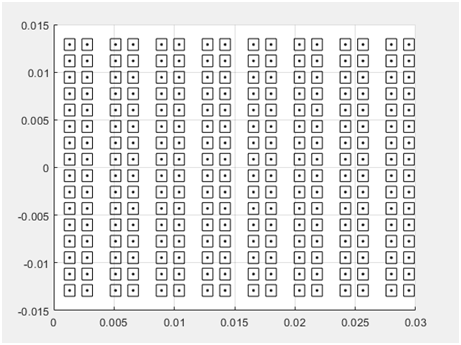
\includegraphics{pic1.png} 
\end{center}
\end{figure}

Информация о детекторе получена из \cite{source1} и \cite{source2}.


Угол между направлением камеры-обскуры и направлением на центр (между $8$ и $9$ лучами): $$ang = \arccos\left(\frac{708^2 + 720^2 - 31^2}{2\cdot 708\cdot 720}\right)$$
\vspace{1mm}

Положение края детектора ($1-$го столбца) (в кординатах $$XY):\;spd\_start=(0,-0.708)$$
\vspace{1mm}

Положение $16-$го столбца (в координатах $XY):$
$$spd\_end=(0.72\cdot\sin(ang),0.72\cdot(-\cos( ang))=(0.002886-0.7194)$$
\vspace{1mm}

Вектор направления камеры-обскуры в экваториальной плоскости (в координатах $XY):$
$$spd\_vect=\frac{spd_{end}-spd_{start}}{\|spd_{end}-spd_{start}\|}= (0.0015,-0.3685)$$
\vspace{1mm}

Шаг между столбцами в плоскости детектора, 2 числа («малый» и «большой» шаги): 
$$spd\_xy\_step=(2.3375 - 0.88,3.81 - 2.3375 + 0.88)\cdot 10^{-3}=(0.0015,0.0024)$$
\vspace{1mm}

Центр детектора (в координатах $XY):$
$$pp=spd_{start}+spd_{vect}\frac{\left(spd_{xy_{step(1)}}+spd_{xy_{step(2)}}\right)\cdot 8+0.52\cdot 1e-03}{2}=(0.00144,-0.7137)$$
\vspace{1mm}

Отступ Апертуры от центра детектора: 
$$aperture\_xy\_offset = 0.0395$$
\vspace{1mm}

Координата апертуры (в плоскости $XY):$ 
\vspace{-2mm}
\begin{multline*}
aperture\_xy =(pp(1) - spd\_vect(2) * aperture\_xy\_offset,\\   pp(2) + spd\_vect(1) * aperture\_xy\_offset) = (0.0290,-0.6770)
\end{multline*}
\vspace{1mm}

$spd\_xz$ – устройство детектора в меридиональной плоскости
\vspace{1mm}

$spd\_z\_start=\frac{27.52-0.49}{2}1e-03=0.0135$
\vspace{1mm}

$spd\_z\_step= -1.72 \cdot 1e-03= -0.0017$
\vspace{1mm}

$spd\_xy=spd\_start+spd\_vect\left(\frac{spd\_xy\_step(2)}{2}+0.26\cdot 1e-03\right)=(0.0013,-0.7085)$

\subsection{Нахождение сечения плазмы плоскостью $\mathbf{x = H}$}
Плазма представляется как фигура вращения. Роль образующей выполняет сетка разбиения сепаратрисы. Для каждого вертикального ряда пикселей детектора вычисляется прямая, проходящая через этот пиксель и апертуру детектора. После чего вычисляет $H$ - расстояние от центра токамака до прямой.

Сечение плазмы плоскость $x = H.$ Далее каждый элемента сетки представляется как фигура вращения, ось вращения совпадает с осью токамака, образующая – текущий элемент сетки. Для этой фигуры рассчитывается сечение плоскость x=H.
В этом сечении для каждого пикселя в вертикальном ряду вычисляется прямая, проходящая через центр пикселя и апертуру детектора.

Далее для ищутся пересечения прямой и элементов сетки, и по точкам пересечений вычисляются длины хорд.



\section{Реализация}
Все задания были выполнены на языке программирования $Matlab$ в среде разработки $MATLAB R2014b$ \hfill \cite{1}

Данные из фала считаны функцией "gfile\_extractor\_1t" \hfill\cite{2}

Радиус кривизны вычислялся по $3$ точкам (как радиус окружности, описанной вокруг треугольника)

$R(i)$ вычисляется по трём точкам: $A = p(i-1), B = p(i), C = p(i+1),$ где $p\;\--$ точки сепаратрисы

Для крайних точек сепаратрисы учитывается её замкнутость

Данные о расположении и параметрах детектора взяты пособия к лабораторной работе \cite{source2}

\section{Результаты}

\begin{figure}[H]
\begin{center}
\caption{График сепаратрисы и магнитной оси }
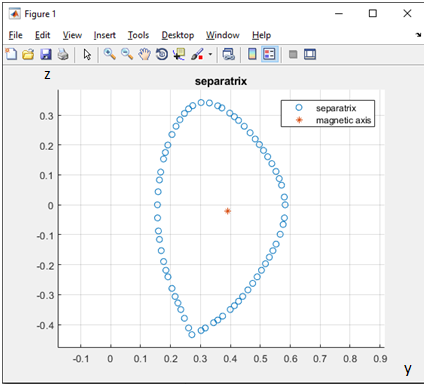
\includegraphics{pic2.png} 
\end{center}
\end{figure}

\begin{figure}[H]
\begin{center}
\caption{Разбиение сепаратрисы}
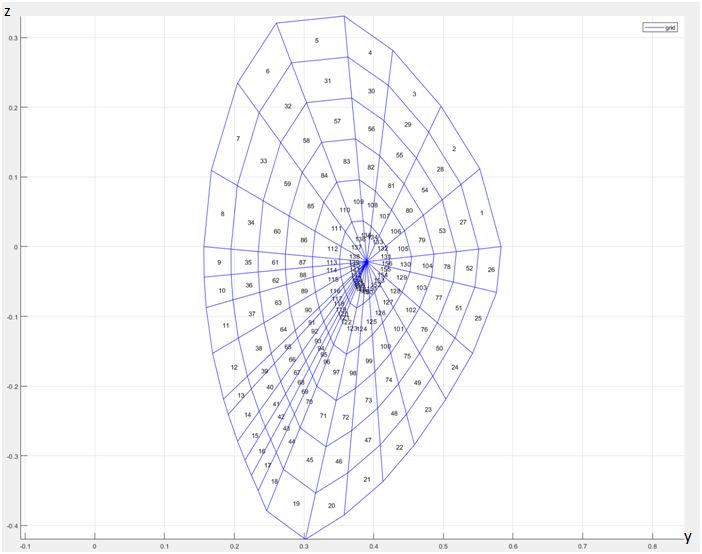
\includegraphics{pic3.png} 
\end{center}
\end{figure}


\begin{figure}[H]
\begin{center}
\caption{график положения сечений}
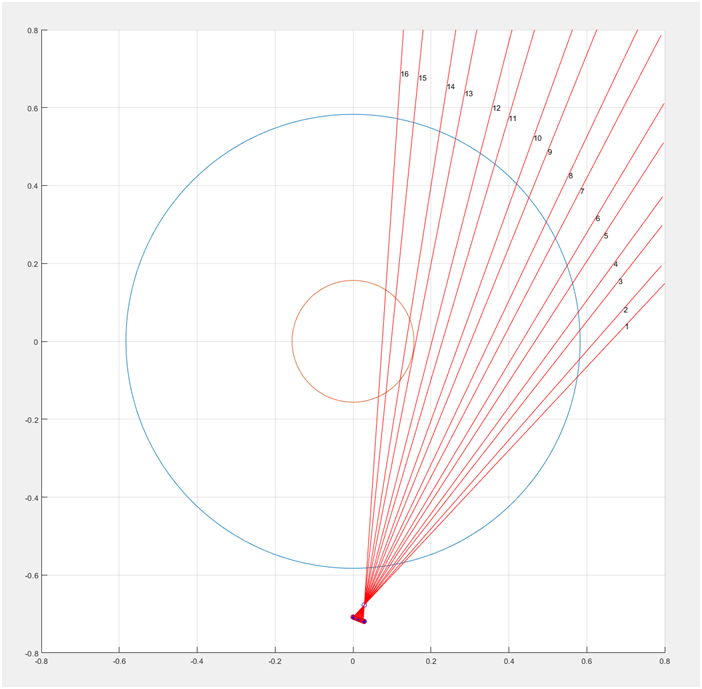
\includegraphics{pic4.png} 
\end{center}
\end{figure}

\begin{figure}[H]
\begin{center}
\caption{график положения лучей для 16 столбца детектора}
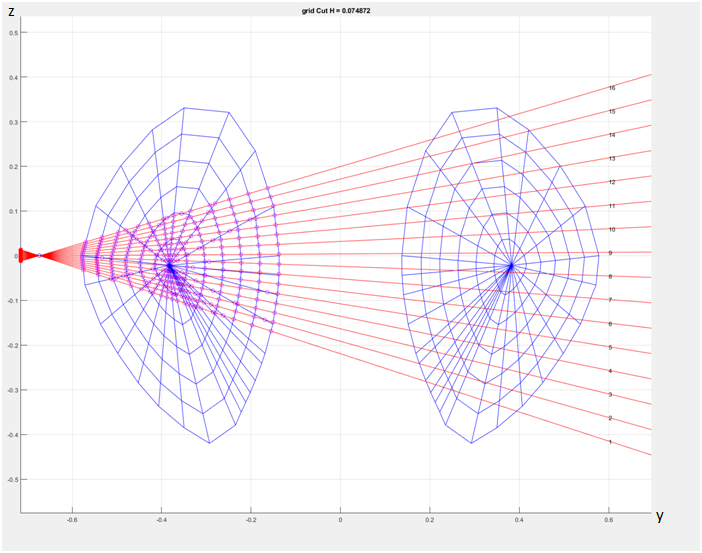
\includegraphics{pic5.png} 
\end{center}
\end{figure}

Сечения для всех $16-$ти столбцов:

\begin{figure}[H]
\begin{center}
\caption{Сечение 1}
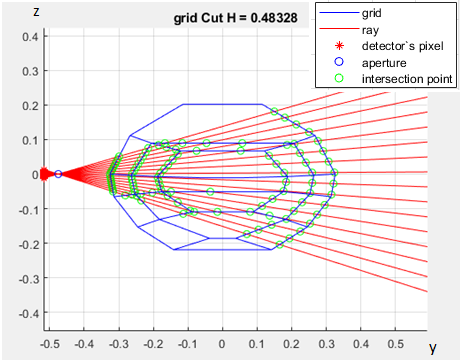
\includegraphics{pic6.png} 

\caption{Сечение 2}
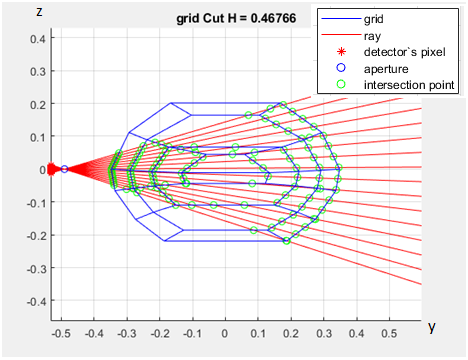
\includegraphics{pic7.png} 
\end{center}
\end{figure}


\begin{figure}[H]
\begin{center}
\caption{Сечение 3}
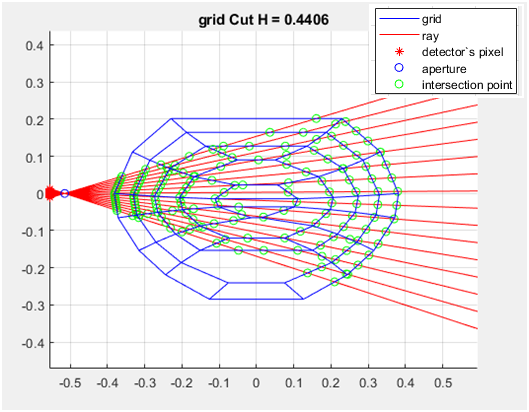
\includegraphics{pic8.png} 

\caption{Сечение 4}
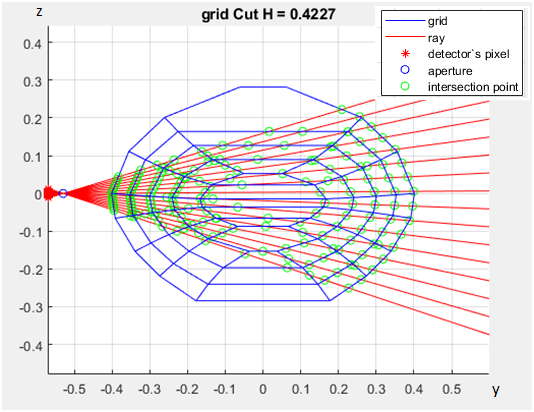
\includegraphics{pic9.png} 
\end{center}
\end{figure}


\begin{figure}[H]
\begin{center}
\caption{Сечение 5}
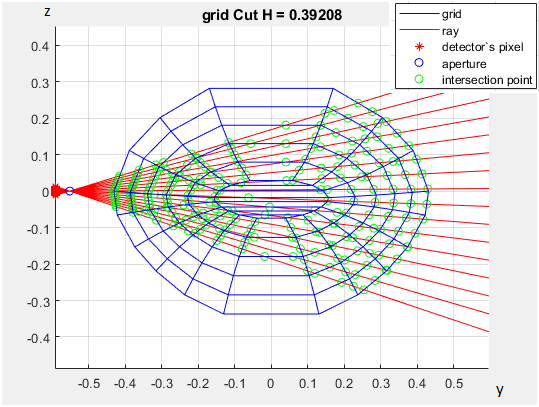
\includegraphics{pic10.png} 

\caption{Сечение 6}
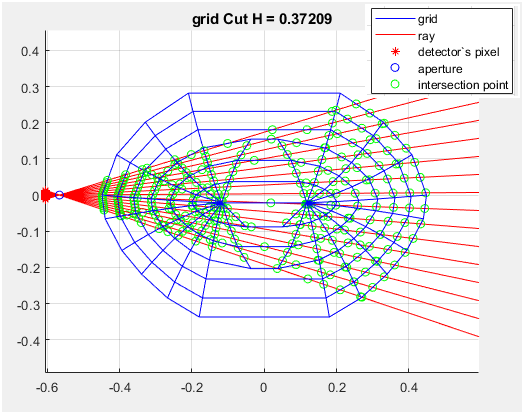
\includegraphics{pic11.png} 
\end{center}
\end{figure}


\begin{figure}[H]
\begin{center}
\caption{Сечение 7}
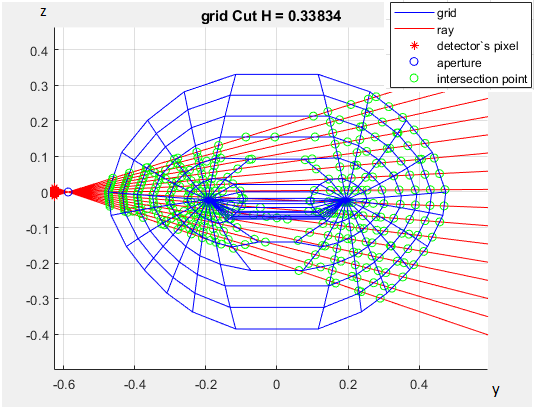
\includegraphics{pic12.png} 

\caption{Сечение 8}
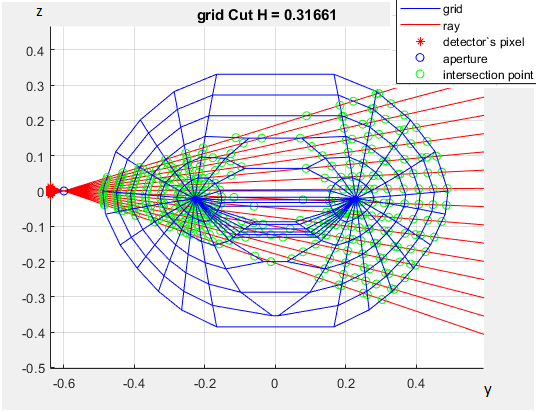
\includegraphics{pic13.png} 
\end{center}
\end{figure}


\begin{figure}[H]
\begin{center}
\caption{Сечение 9}
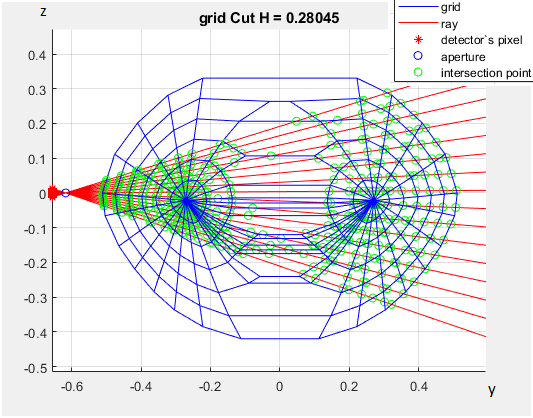
\includegraphics{pic14.png} 

\caption{Сечение 10}
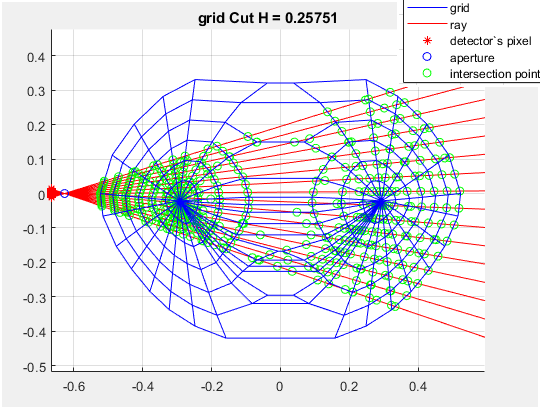
\includegraphics{pic15.png} 
\end{center}
\end{figure}


\begin{figure}[H]
\begin{center}
\caption{Сечение 11}
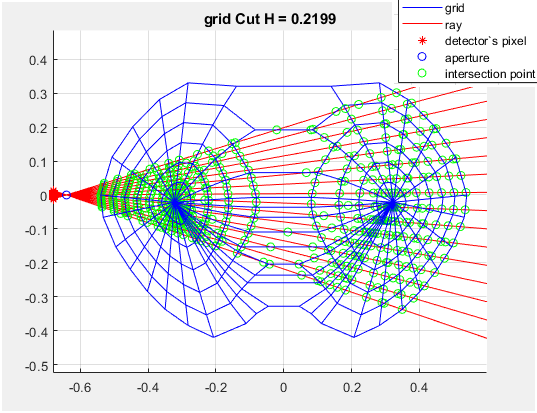
\includegraphics{pic16.png} 

\caption{Сечение 12}
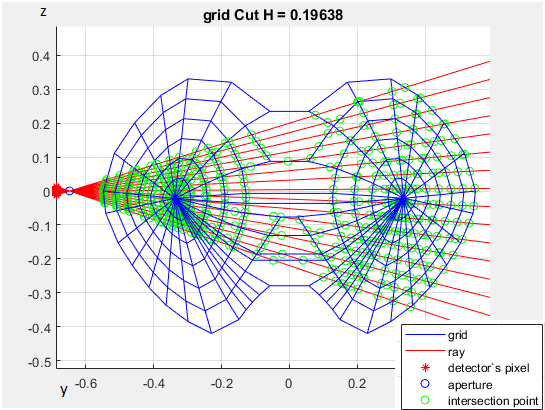
\includegraphics{pic17.png} 
\end{center}
\end{figure}


\begin{figure}[H]
\begin{center}
\caption{Сечение 13}
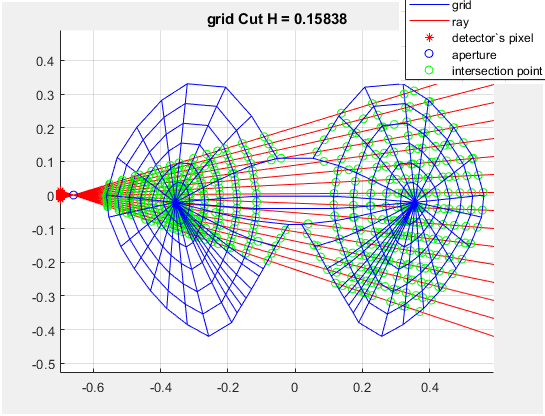
\includegraphics{pic18.png} 

\caption{Сечение 14}
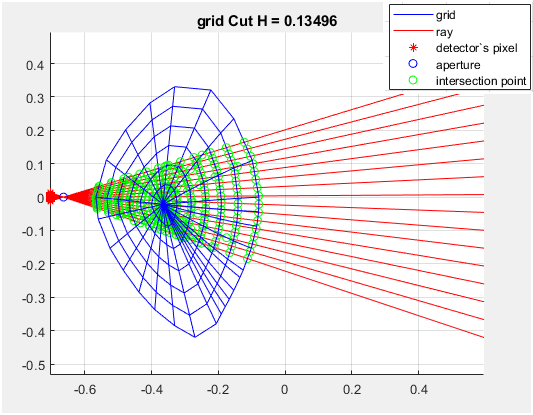
\includegraphics{pic19.png} 
\end{center}
\end{figure}


\begin{figure}[H]
\begin{center}
\caption{Сечение 15}
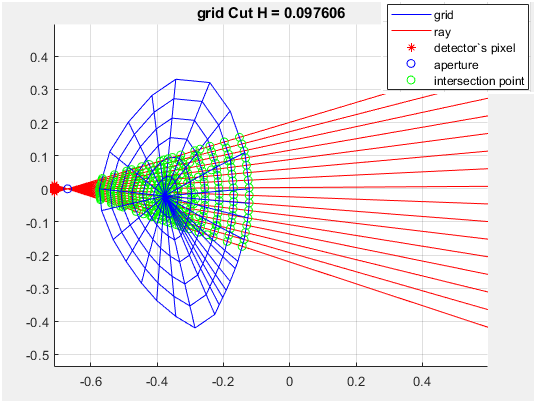
\includegraphics{pic20.png} 

\caption{Сечение 16}
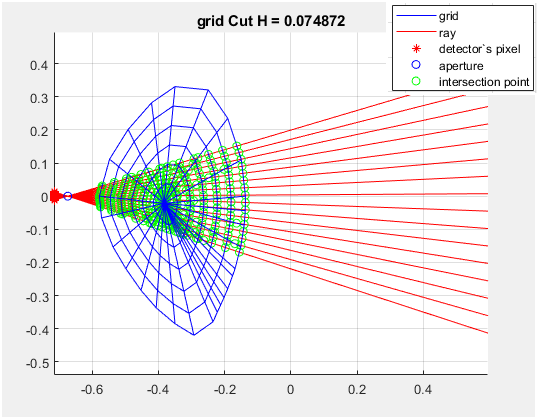
\includegraphics{pic21.png} 
\end{center}
\end{figure}

\begin{figure}[H]
    \centering
    \caption{Разреженная матрица}
    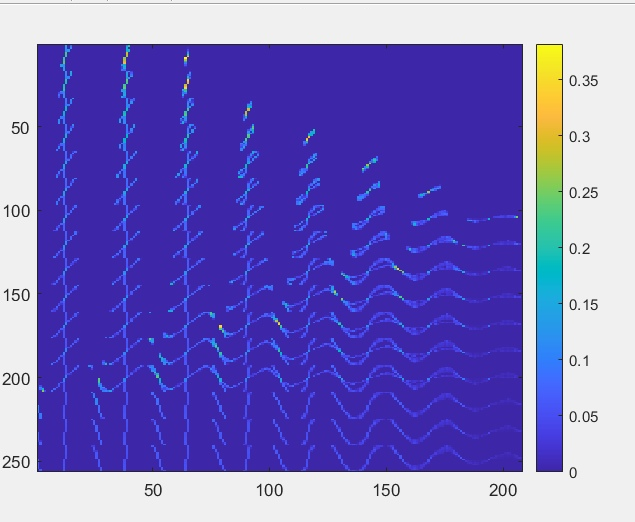
\includegraphics{pic22.png}
\end{figure}

\section{Обсуждение}
На сечениях $14,$ $15,$ $16$ плоскость сечения H меньше самой левой точки сепаратрисы, следовательно, область получается двусвязной.
В случае двусвязной области считаем, что луч упирается в центральную ось токамака, и учитываем только левую (ближайшую к детектору) область.
	
СЛАУ представляет собой матрицу $256\times N,$ где N – это количество элементов разбиения.
Каждая строка матрицы отвечает за свой луч, притом коэффициенты для каждого элемента разбиения – сумма длин хорд.


\begin{thebibliography}{}
    \bibitem{1}  Документация по Матлаб: https://www.mathworks.com/help/

    \bibitem{2} Код функции g\_file\_extractor\_1t: https://cloud.mail.ru/public/5o3T/4G4dD71hL
    
    \bibitem{source}
    Пособие к Лабораторным работам https://cloud.mail.ru/public/4ra6/5wwqBzMBC/LabPractics.pdf
    
    \bibitem{source1}
    Пособие к Лабораторным работам «Построение матриц СЛАУ» https://vk.com/doc38035266\_528474113?hash=8c9ddc720dfadef7b6\&dl=48b180ef19a7dc0f33
    
    \bibitem{source2}
    Выпуская квалификационная работа бакалавра «Исследование разрешимости обратных задач с помощью распознающего функционала» https://cloud.mail.ru/public/4ra6/5wwqBzMBC/2019\%20Затылкин\%20бакалавр.pdf
\end{thebibliography}

\section{Приложения}

Код отчёта:\; \url{https://github.com/MisterProper9000/computing-complex/blob/lab-4-linear-system/Lab_4(linear\_system)/texReport/lab4.tex}

Код лаборатрной:\; \url{https://github.com/MisterProper9000/computing-complex/blob/lab-4-linear-system/Lab_4(linear\_system)}



\end{document}
